\documentclass[11pt,a4paper]{article}
\usepackage[T1]{fontenc}
\usepackage[utf8]{inputenc}
\usepackage{lmodern,microtype}
\usepackage[margin=25mm]{geometry}
\usepackage{amsmath,amssymb,amsthm,mathtools}
\usepackage{graphicx,booktabs,array,longtable}
\usepackage{xcolor}
\usepackage{enumitem}
\usepackage{xurl}
\usepackage{hyperref}
\usepackage{bookmark}
\usepackage{fancyhdr}
\hypersetup{colorlinks=true,linkcolor=blue!45!black,citecolor=blue!45!black,urlcolor=blue!55!black,pdftitle={Sharp constants for dyadic pole detection},pdfauthor={Research report prepared with ChatGPT for Vladimir Reshetnikov}}
\pagestyle{fancy}\fancyhf{}\fancyhead[L]{\small Sharp constants for dyadic pole detection}\fancyhead[R]{\small 26 November 2026}\fancyfoot[C]{\thepage}
\setlength{\headheight}{14pt}
\setlength{\emergencystretch}{2em}
\setlist{itemsep=3pt,topsep=5pt}
\newtheorem{theorem}{Theorem}[section]
\newtheorem{proposition}[theorem]{Proposition}
\newtheorem{lemma}[theorem]{Lemma}
\newtheorem{corollary}[theorem]{Corollary}
\theoremstyle{definition}\newtheorem{definition}[theorem]{Definition}
\theoremstyle{remark}\newtheorem{remark}[theorem]{Remark}
\newcommand{\C}{\mathbb C}\newcommand{\R}{\mathbb R}
\newcommand{\Res}{\operatorname{Res}}
\newcommand{\Rea}{\operatorname{Re}}
\newcommand{\Ima}{\operatorname{Im}}
\newcommand{\M}{\mathcal M}
\newcommand{\ord}{\operatorname{ord}}
\newcommand{\repo}{\texttt{lsernau/grh-lean}}
\newcommand{\sha}{\nolinkurl{72fead102f663d5c7a407964a13dc0cf9d977207}}
\title{\vspace{-9mm}\textbf{Sharp constants for dyadic pole detection}\\[3mm]\large An extremal theorem motivated by the analytic endpoint of \repo}
\author{Research report prepared for Vladimir Reshetnikov}
\date{26 November 2026}
\begin{document}
\maketitle
\begin{abstract}
We solve an infinite family of extremal problems that arise when one observes a Mellin transform through positive sums at successively doubled shifts. For even $n\ge2$, put $L=2^{n-1}$ and let $r\in(1/2,1)$ solve $r+r^L=1$. We prove
\[
\min_{z\in\C}\max_{0\le j<n}|1+z^{2^j}|=\sqrt{1-r+r^2},
\]
with exactly two minimizers, $r e^{\pm2\pi i/3}$. The proof combines angle doubling in a half-plane with a strictly concave function of logarithmic radius. We give an explicit stability estimate, an asymptotic formula, and the exact three-filter constant, determined by a quartic. A separate polynomial certificate proves quantitative stability in the three-filter case. These constants give sharp worst-case recovery bounds for residues of meromorphic transforms and a filtered version of a classical one-sided Landau criterion. The link with \repo{} is its passage from a smoothed prime remainder to transform poles; no RH or GRH assumption is needed for our extremal theorems. The two-filter case is classical. The infinite even family and the three-filter refinements are proposed original contributions: targeted searches found no prior statements, but do not establish priority.
\end{abstract}
\vspace{2mm}
\noindent\textbf{What is proved here.} Complete analytic proofs, explicit equality cases, sharp noise constants, and exact symbolic certificates.\par
\noindent\textbf{Verification scope.} Source inspection of a pinned GRH repository; independent mathematical cross-checks and executable symbolic checks of this note. No fresh build of the GRH repository and no completed Lean formalization of the new theorems are claimed.
\setcounter{tocdepth}{1}
\tableofcontents
\newpage

\section{What the supplied sources contribute}
\subsection{Scope of the formal result}
We inspected \repo{} at commit \sha. Its exported statements use Mathlib's Riemann zeta function and Dirichlet $L$-functions. They cover RH, nonvanishing of every Dirichlet $L$-function in $\Rea s>1/2$ away from the principal-character pole, and the critical-line statement for zeros in $0<\Rea s<1$, including imprimitive characters. The exact statement file is \texttt{grh/src/Statements.lean}; \texttt{grh/src/Main.lean} supplies the exported proofs \cite{statements,main}.

The reported axioms are \texttt{propext}, \texttt{Classical.choice}, and \texttt{Quot.sound}. The project reports Lean and independent-kernel checks. Its readable edition pins Lean 4.35.0 and Mathlib commit \nolinkurl{56a005855ea17e0b0958f73ec801ae140b0a1679}. This report inspected source and documentation; it did not repeat those full builds or replay checks \cite{readme}.

The supplied Wikipedia article, as retrieved on the report date, describes the November 2026 proof and surveys known consequences and equivalent formulations \cite{wiki}. It served as orientation. The mathematical extraction below is grounded in the repository's definitions and lemmas. In particular, the exported Dirichlet statements do not by themselves supply GRH for general Artin or automorphic $L$-functions.

\subsection{The mechanism we isolate}
The repository's geometric comparison has three inputs: sufficiently short integral forms, enough forms to span a large subspace, and a lower bound on the size of integral forms. A corrected logarithmic covolume is bounded in two ways. The large main contribution cancels, leaving a bound on a prime remainder. The chain length is of order $\sqrt{x}$ \cite{guide,mainineq}.

At the analytic endpoint, for an admissible odd prime $d$ and modulus $q$, the relevant remainder has the form
\begin{equation}\label{eq:prime-remainder}
R_{d,q}(x)=\sum_{\substack{1\le m\le x\\m\equiv1\pmod q}}
\Lambda(m)(1-\chi_d(m))\left(\frac1m-\frac1x\right)
-\frac{\log x}{\varphi(q)}-c_{d,q},
\end{equation}
where $\chi_d(m)=(m/d)$ and the constant is fixed by the logarithmic-derivative normalization. The proof obtains an eventual one-sided estimate of size $x^{-1/2+\varepsilon}$ \cite{onesided}.

Writing $E(t)=R_{d,q}(e^t)$, its transform is
\begin{equation}\label{eq:transform}
F(s)=\int_0^\infty E(t)e^{(1-s)t}\,dt,
\end{equation}
initially in a right half-plane. At $\Rea\rho>0$, $\rho\ne1$, the residue formula involves the difference of zero multiplicities
\begin{equation}\label{eq:arithmetic-residue}
\Res_{s=\rho}F(s)=\frac{\nu_{d,q}(\rho)}{\varphi(q)\rho(1-\rho)},\qquad
\nu_{d,q}(\rho)=\sum_{\chi\bmod q}\ord_\rho L(s,\chi)
-\sum_{\chi\bmod q}\ord_\rho L(s,\chi\chi_d).
\end{equation}
In the critical strip this agrees with the repository's pole-removed \texttt{entireL} convention \cite{primeerror}. A twist-selection argument and a one-sided Landau lemma finish the exclusion of unwanted poles \cite{criterion,landau}.

\subsection{The new question}
A positive combination of shifted values of $E$ remains compatible with a one-sided estimate. But its transform multiplies a residue by a complex factor, which may nearly vanish. How much of a pole can be hidden simultaneously in several observations at doubled shifts? We answer this question exactly for every even number of observations, and also for three observations.

This is a mathematical extension of the \emph{analytic interface} in the proof. It does not generalize the theta-lift construction or establish another unresolved number-theoretic conjecture. Its new content is the exact extremal geometry and the resulting quantitative control of cancellation.

\section{An exact theorem for every even number of filters}
\begin{definition}
For an integer $n\ge1$, define
\[
\M_n(z)=\max_{0\le j<n}|1+z^{2^j}|,\qquad
c_n=\inf_{z\in\C}\M_n(z).
\]
The exponents are $1,2,4,\ldots,2^{n-1}$. The word \emph{dyadic} refers to this successive doubling.
\end{definition}

\begin{theorem}[Exact even family]\label{thm:even}
Let $n\ge2$ be even, $L=2^{n-1}$, and let $r_n\in(1/2,1)$ be the unique solution of
\begin{equation}\label{eq:r-def}
r_n+r_n^L=1.
\end{equation}
Then
\begin{equation}\label{eq:even-value}
\boxed{\ c_n=\sqrt{1-r_n+r_n^2}\ },
\end{equation}
and the full set of minimizers is
\begin{equation}\label{eq:even-minimizers}
\boxed{\ z=r_n e^{2\pi i/3}\quad\hbox{or}\quad z=r_n e^{-2\pi i/3}.\ }
\end{equation}
\end{theorem}

The case $n=2$ gives $r_2=(\sqrt5-1)/2$ and $c_2=\sqrt{3-\sqrt5}$. This exact two-polynomial problem appears in the 1968 collection \emph{Contests in Higher Mathematics}, Section 3.3, Problem 2 \cite{contests}. We make no novelty claim for that case. The assertion here is the extension to every even $n$, together with the stability analysis below.

\subsection{The logarithmic-radius lemma}
\begin{lemma}[A symmetric concave angle function]\label{lem:concavity}
For $0<d<1$, set
\[
A_d(v)=\arccos\left(\frac{v+d/v}{2}\right)
\]
where $v>0$ and $v+d/v\le2$. The domain of
\[
g_d(u)=A_d(e^u)
=\arccos\bigl(\sqrt d\,\cosh(u-\tfrac12\log d)\bigr)
\]
is a closed interval. On that interval it is continuous and strictly concave, and
\begin{equation}\label{eq:symmetry}
g_d(u)=g_d(\log d-u),\qquad A_d(v)=A_d(d/v).
\end{equation}
On the interior,
\begin{equation}\label{eq:g-second}
g_d''(u)=
-\frac{\sqrt d(1-d)\cosh(u-\tfrac12\log d)}
{\left(1-d\cosh^2(u-\tfrac12\log d)\right)^{3/2}}
\le-\sqrt{\frac d{1-d}}.
\end{equation}
\end{lemma}
\begin{proof}
The domain is the interval
$|u-\frac12\log d|\le\operatorname{arcosh}(d^{-1/2})$.
The symmetry follows from the evenness of $\cosh$. Differentiating twice gives \eqref{eq:g-second}. Since $\cosh\ge1$ and the denominator is at most $(1-d)^{3/2}$, the stated uniform bound follows. Strict concavity extends to the closed interval by continuity.
\end{proof}

\subsection{Proof of the exact even family}
\begin{proof}[Proof of Theorem~\ref{thm:even}]
Existence and uniqueness of $r=r_n$ follow because $v+v^L$ is strictly increasing, is less than $1$ at $v=1/2$, and exceeds $1$ at $v=1$. Put
\[
c=\sqrt{1-r+r^2},\qquad d=1-c^2=r(1-r)=r^{L+1}.
\]
We first show that the displayed candidates attain $c$. If $z=r e^{\pm2\pi i/3}$, successive squaring alternates the two arguments $\pm2\pi/3$. Hence
\[
|1+z^{2^j}|^2=1-r^{2^j}+r^{2^{j+1}}.
\]
Every $r^{2^j}$ lies in $[r^L,r]=[1-r,r]$. The convex function $v\mapsto1-v+v^2$ takes the same value $1-r+r^2$ at these two endpoints, so all the displayed values are at most $c^2$, with equality at the first and last. Thus $c_n\le c$.

Now suppose $\M_n(z)\le c$. Since $c<1$, $z\ne0$ and every $z^{2^j}$ has negative real part. Write $v=|z|$ and
\[
\alpha_j=\left|\operatorname{Arg}(-z^{2^j})\right|\in[0,\pi/2).
\]
For consecutive iterates both in the left half-plane, angle doubling gives
\begin{equation}\label{eq:angle-recurrence}
\alpha_{j+1}=\pi-2\alpha_j.
\end{equation}
Indeed, if the argument of an iterate is $\pi\pm\alpha_j$, its square has argument $\pm2\alpha_j$; negativity of the next real part forces $\alpha_j>\pi/4$ and gives the formula. Iteration yields
\[
\alpha_j=\frac\pi3+(-2)^j\left(\alpha_0-\frac\pi3\right).
\]
Because $n$ is even, $n-1$ is odd and therefore
\begin{equation}\label{eq:angle-endpoints}
L\alpha_0+\alpha_{n-1}=(L+1)\frac\pi3.
\end{equation}

The inequality $|1+z^{2^j}|\le c$ is equivalent to
\[
\cos\alpha_j\ge\frac{v^{2^j}+d/v^{2^j}}2.
\]
Consequently $\alpha_j\le A_d(v^{2^j})$. In particular the two endpoint radii are in the domain of $A_d$. Use the symmetry in Lemma~\ref{lem:concavity}, then Jensen's inequality with weights $L/(L+1)$ and $1/(L+1)$:
\begin{align*}
\frac\pi3
&=\frac{L\alpha_0+\alpha_{n-1}}{L+1}\\
&\le\frac{L A_d(v)+A_d(v^L)}{L+1}\\
&=\frac{L g_d(\log v)+g_d(\log d-L\log v)}{L+1}\\
&\le g_d\left(\frac{\log d}{L+1}\right)
=A_d(r)=\arccos\left(\frac{r+r^L}{2}\right)=\frac\pi3.
\end{align*}
Both arguments of $g_d$ belong to its convex domain, so this use of Jensen is valid, including endpoints.

Every inequality is an equality. Strict concavity implies
$\log v=\log d-L\log v$, whence $v=r$. Equality in the first angular bound gives $\alpha_0=\pi/3$. Thus $z=r e^{\pm2\pi i/3}$. Those two points have $\M_n(z)=c$, so no value below $c$ is possible and there are no other minimizers.
\end{proof}

\begin{remark}[Why the parity hypothesis matters]
For odd $n$, the endpoint relation has a minus sign:
$L\alpha_0-\alpha_{n-1}=(L-1)\pi/3$.
The positive-weight Jensen argument above no longer applies. Section~\ref{sec:triple} solves $n=3$ and shows that the even-family formula would give the wrong value there.
\end{remark}

\section{Stability and the limiting constant}
\subsection{An explicit estimate for near minimizers}
\begin{theorem}[Stability in the even family]\label{thm:even-stability}
Let $n\ge2$ be even and $L=2^{n-1}$. Suppose $\M_n(z)\le B<1$. Define
\[
d=1-B^2,\qquad r_*=d^{1/(L+1)},\qquad
\kappa=\frac{\sqrt d}{B},\qquad
\Delta=A_d(r_*)-\frac\pi3.
\]
Then $\Delta\ge0$, and
\begin{equation}\label{eq:radial-stability}
\boxed{\ \left|\log\frac{|z|}{r_*}\right|
\le\sqrt{\frac{2\Delta}{\kappa L}}.\ }
\end{equation}
If $\alpha=|\operatorname{Arg}(-z)|$, then also
\begin{equation}\label{eq:angular-stability}
A_d(|z|)-\frac{L+1}{L}\Delta\le\alpha\le A_d(|z|).
\end{equation}
In particular, as $B\downarrow c_n$, all such $z$ approach the two minimizers of Theorem~\ref{thm:even}.
\end{theorem}
\begin{proof}
Repeat the angular argument with this $d$. The endpoint Jensen inequality implies $A_d(r_*)\ge\pi/3$, so all the quantities are defined and $\Delta\ge0$.

Equation~\eqref{eq:g-second} says that $g_d$ is $\kappa$-strongly concave. For two arguments $u_1,u_2$ and weight $\lambda$, its Jensen gap is at least
$\frac\kappa2\lambda(1-\lambda)(u_1-u_2)^2$; this follows by applying ordinary concavity to $g_d(u)+\kappa u^2/2$.
Use $u_1=\log|z|$, $u_2=\log d-Lu_1$, and $\lambda=L/(L+1)$. The gap is at least
\[
\frac{\kappa L}{2}\left(\log|z|-\frac{\log d}{L+1}\right)^2.
\]
The weighted average is at least $\pi/3$, so the gap is at most $\Delta$. This proves \eqref{eq:radial-stability}.

The two nonnegative angular slacks satisfy
\[
L\bigl(A_d(|z|)-\alpha_0\bigr)
+\bigl(A_d(|z|^L)-\alpha_{n-1}\bigr)\le(L+1)\Delta.
\]
Discarding the second term gives \eqref{eq:angular-stability}. At $B=c_n$ we have $r_*=r_n$ and $\Delta=0$; continuity completes the last assertion.
\end{proof}

\subsection{Asymptotics}
\begin{proposition}\label{prop:asymptotic}
Along even $n\to\infty$, with $L=2^{n-1}$ and $W(L)>0$ defined by $W(L)e^{W(L)}=L$,
\begin{align}
r_n&=1-\frac{W(L)}L+O\left(\frac{W(L)^2}{L^2}\right),\label{eq:r-asymptotic}\\
c_n&=1-\frac{W(L)}{2L}+O\left(\frac{W(L)^2}{L^2}\right).
\end{align}
In particular $c_n\uparrow1$ along the even indices.
\end{proposition}
\begin{proof}
Put $\varepsilon=1-r_n=r_n^L$ and $t=L\varepsilon$. Taking logarithms gives
\[
\log(t/L)=L\log(1-t/L).
\]
Since $-\log(1-u)\ge u$, this implies $t+\log t\le\log L$, hence $t\le W(L)$. Thus $t/L\to0$, and Taylor's formula gives
\[
t+\log t=\log L+O(t^2/L).
\]
The derivative of $u+\log u$ is at least $1$, so
$t=W(L)+O(W(L)^2/L)$. This proves \eqref{eq:r-asymptotic}. Next,
$c_n=\sqrt{1-\varepsilon+\varepsilon^2}=1-\varepsilon/2+O(\varepsilon^2)$.
The defining equation shows that $r_n$ increases with $L$; on $(1/2,1)$ the function $1-r+r^2$ increases. This proves monotonicity.
\end{proof}

\begin{table}[ht]
\centering
\begin{tabular}{rrrr}
\toprule
Filters $n$ & Largest exponent $2^{n-1}$ & Exact-form $c_n$ (decimal) & $1/c_n$ (decimal)\\
\midrule
2 & 2 & 0.874032048898 & 1.144122805635\\
3 & 4 & 0.882003267585 & 1.133782647697\\
4 & 8 & 0.920395115469 & 1.086489903296\\
6 & 32 & 0.963810398091 & 1.037548465944\\
8 & 128 & 0.986468300101 & 1.013717318536\\
10 & 512 & 0.995466276153 & 1.004554372112\\
12 & 2048 & 0.998574881565 & 1.001427152296\\
\bottomrule
\end{tabular}
\caption{Sharp lower gains. The three-filter row uses Theorem~\ref{thm:triple}. Full-precision values are regenerated in \texttt{data/constants.csv}; the recovery factors are rounded here.}
\label{tab:constants}
\end{table}

\section{The exact three-filter problem}\label{sec:triple}
\begin{theorem}[Three filters]\label{thm:triple}
Let $\tau$ be the unique root in $(1/2,3/5)$ of
\begin{equation}\label{eq:quartic}
q(t)=t^4-2t^2-3t+2=0.
\end{equation}
Then
\begin{equation}\label{eq:c3}
\boxed{\ c_3=\sqrt{\tau+\tau^2}=0.8820032675847058285\ldots\ },
\end{equation}
and its only minimizers are
\begin{equation}\label{eq:z3}
z=\frac{\tau^2-1}{2}\ \pm\ \frac{i\sqrt{\tau+1}}2.
\end{equation}
At both points, all three quantities $|1+z|,|1+z^2|,|1+z^4|$ are equal.
\end{theorem}

\subsection{Reduction to two intervals}
\begin{proof}
Write $x=\Rea z$, $t=|z|^2$, and
\[
A=|1+z|^2=1+2x+t,\quad
B=|1+z^2|^2=(1-t)^2+4x^2,
\]
\[
C=|1+z^4|^2=(1-t^2)^2+4(2x^2-t)^2.
\]
Consider a proposed upper bound $M<1$ for $\max(A,B,C)$. The bound on $A$ forces $x<0$. At fixed $t$, increase $a=-x\ge0$ until $B=M$. This is geometrically permissible: $a\le\sqrt t$, and at $a=\sqrt t$ one has $B=(1+t)^2>M$. Increasing $a$ decreases $A$. It also decreases $C$ throughout $B\le M$, because
\[
C=(1-t^2)^2+(B-1-t^2)^2,\qquad B-1-t^2<0.
\]
Consequently feasibility at this $t$ is equivalent to feasibility at
\[
a=\frac12\sqrt{M-(1-t)^2}.
\]
At that endpoint the conditions $A\le M$ and $C\le M$ become, respectively,
\begin{equation}\label{eq:qM}
Q_M(t)\ge0,\quad Q_M(t^2)\ge0,\qquad
Q_M(v)=-2v^2+2Mv+3M-M^2-2.
\end{equation}
For the first equivalence we square a nonnegative right-hand side $1+t-M$; the condition $Q_M(t)\ge0$ itself guarantees the needed square root exists.

The discriminant condition requires $M\ge3-\sqrt5$. For
$3-\sqrt5\le M<1$, the roots of $Q_M$ are
\[
\ell(M)=\frac{M-\sqrt{-M^2+6M-4}}2,\qquad\nu(M)=\frac{M+\sqrt{-M^2+6M-4}}2,
\]
with $0<\ell(M)\le\nu(M)<1$. Thus \eqref{eq:qM} is equivalent to
\[
t\in[\ell,\nu],\quad t^2\in[\ell,\nu],
\]
which, since $0<t<1$, is feasible exactly when
\begin{equation}\label{eq:root-touch}
\ell(M)\le\nu(M)^2.
\end{equation}
On this interval $\ell$ strictly decreases and $\nu$ strictly increases: away from its left endpoint, the derivative of the square-root term is $(3-M)/\sqrt{-M^2+6M-4}>1$. At $M=3-\sqrt5$ the inequality \eqref{eq:root-touch} fails; as $M\uparrow1$ it holds strictly. There is therefore exactly one first feasible value, with $\ell=\nu^2$.

Put $\tau=\nu$ at that value. Since $\ell+\nu=M$, we have $M=\tau+\tau^2$. Substitution in $Q_M(\tau)=0$ gives $q(\tau)=0$. The polynomial $q$ is strictly decreasing on $(0,1)$, because $q'(t)=4t(t^2-1)-3<0$, and its signs at $1/2$ and $3/5$ are opposite. This identifies $\tau$ uniquely.

At the threshold, $t=\tau$ is forced. At the endpoint where $B=M$ one also has $A=M$; any smaller value of $a$ would violate $A\le M$. Hence the original point has $A=B=M$, which gives $x=(\tau^2-1)/2$, and the quartic implies
\[
x^2=\frac{3\tau-1}{4},\qquad
(\Ima z)^2=\tau-x^2=\frac{\tau+1}{4}.
\]
These yield exactly \eqref{eq:z3}; substitution gives $A=B=C=\tau+\tau^2$. They attain a value below $1$, so no omitted case $M\ge1$ affects the minimum.
\end{proof}

\subsection{A second certificate and a stronger stability conclusion}
The next proof certificate is independent of the interval-touching argument. It is useful because its identities involve only polynomials and rational coefficients, except for the algebraic parameter $\tau$.

\begin{proposition}[Polynomial certificate and stability]\label{prop:triple-stability}
Let $x_0=(\tau^2-1)/2$, $M_0=\tau+\tau^2$, and
$\omega=4\tau(1-\tau^2)>0$. For every $z\in\C$ satisfying
$\M_3(z)^2\le M_0+\varepsilon<1$,
\begin{equation}\label{eq:triple-stability}
\boxed{\ (\Rea z-x_0)^2+(|z|^2-\tau)^2
\le(\omega+3)\varepsilon.\ }
\end{equation}
\end{proposition}
\begin{proof}
Treat $x$ and $u=|z|^2$ as independent real variables and set
\begin{align*}
A(x,u)&=1+2x+u,\\
B(x,u)&=1+4x^2-2u+u^2,\\
C(x,u)&=1+16x^4-16x^2u+2u^2+u^4,\\
P(x,u)&=\omega A(x,u)+2B(x,u)+C(x,u).
\end{align*}
On the convex set $D=\{u\ge0,\ 2x+u\le0\}$, the Hessian is
\[
H=\begin{pmatrix}
192x^2-32u+16&-32x\\-32x&12u^2+8
\end{pmatrix}.
\]
Since $x^2\ge u^2/4$ on $D$, its first diagonal entry minus $2$ is at least
$48u^2-32u+14>0$. Moreover,
\begin{align}\label{eq:hessian-sos}
\det(H-2I)
={}&(2304u^2+128)(x^2-u^2/4)\\
&+64u^2(3u-1)^2+136(u-12/17)^2+276/17>0.\nonumber
\end{align}
Thus $H\succ2I$ throughout $D$.

Reduction modulo $q(\tau)=0$ gives
\[
\nabla P(x_0,\tau)=0,\qquad
P(x_0,\tau)=(\omega+3)M_0.
\]
The point $(x_0,\tau)$ lies in $D$, because $2x_0+\tau=M_0-1<0$. Integrating the Hessian along a line segment in $D$ yields
\[
P(x,u)\ge(\omega+3)M_0+(x-x_0)^2+(u-\tau)^2.
\]
The hypothesis on $z$ gives $(x,u)\in D$ and
$P(x,u)\le(\omega+3)(M_0+\varepsilon)$. Combining the two inequalities proves \eqref{eq:triple-stability}. All polynomial identities in this argument are checked exactly by the supplied Sympy script.
\end{proof}

\begin{figure}[ht]
\centering
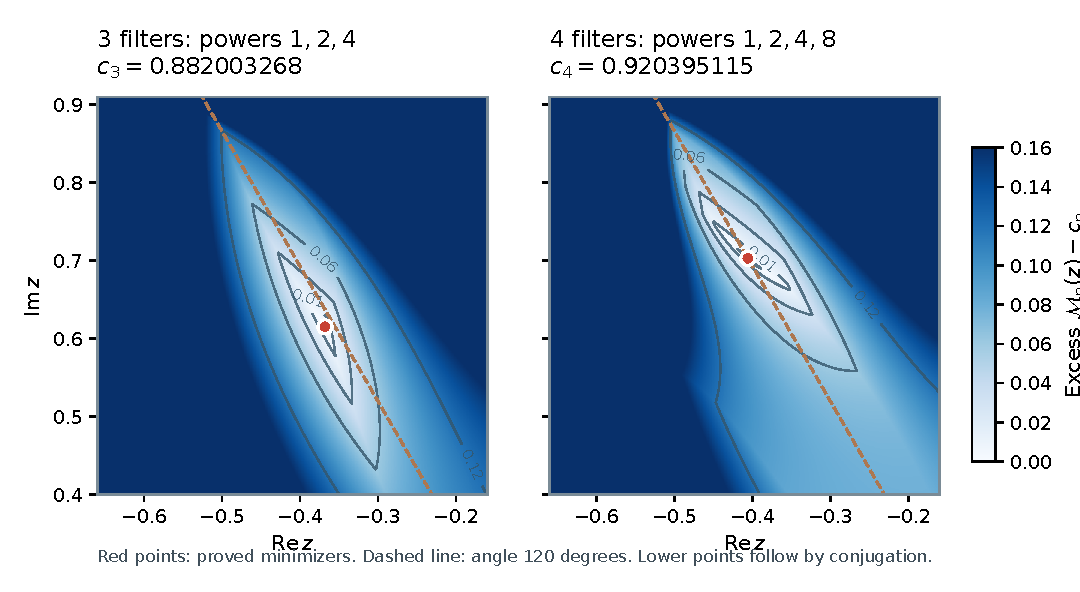
\includegraphics[width=\linewidth]{figures/extremal_geometry.pdf}
\caption{The upper conjugate minimizers for three and four dyadic filters. Contours show $\M_n(z)$; the marked minimizers and minimum values are proved analytically. The numerical drawing is illustrative. The three-filter optimum leaves the angle $2\pi/3$, while the four-filter optimum lies exactly on it.}
\label{fig:geometry}
\end{figure}

\section{From complex polynomials to visible transform poles}
\subsection{The exact shift formula}
Let $E:[0,\infty)\to\R$ be locally integrable and of exponential order. Let $F$ be its transform \eqref{eq:transform}, initially defined sufficiently far to the right, with a meromorphic continuation to a domain of interest. Fix $a,h>0$ and put $k_j=2^j$. Define the positive two-term observations
\begin{equation}\label{eq:filtered-E}
E_j(t)=E(t)+a^{k_j}E(t+k_jh),\qquad 0\le j<n.
\end{equation}
Let $F_j$ denote their transforms, and write
\[
z(s)=a e^{h(s-1)},\qquad
H_j(s)=\int_0^{k_jh}E(u)e^{(1-s)u}\,du.
\]
A change of variable gives the exact identity
\begin{equation}\label{eq:shift-identity}
\boxed{\ F_j(s)=(1+z(s)^{k_j})F(s)-z(s)^{k_j}H_j(s).\ }
\end{equation}
Each $H_j$ is entire, by differentiation under an integral over a compact interval. Thus the endpoint correction must be retained for transform values, but contributes no pole.

\begin{theorem}[Sharp residue visibility]\label{thm:residue}
Suppose $F$ has at most a simple pole at $\rho$, with residue $R$. Write $R_j=\Res_{s=\rho}F_j(s)$. Then
\[
R_j=(1+z(\rho)^{2^j})R,
\]
and, for even $n\ge2$ or $n=3$,
\begin{equation}\label{eq:residue-gain}
\boxed{\ \max_{0\le j<n}|R_j|\ge c_n|R|.\ }
\end{equation}
The constants in Theorems~\ref{thm:even} and \ref{thm:triple} are the largest possible constants in this assertion, even for transforms of real smooth functions.
\end{theorem}
\begin{proof}
Take residues in \eqref{eq:shift-identity} and apply the corresponding extremal theorem.
For sharpness choose a nonreal $\rho$ such that $a e^{h(\rho-1)}$ is an extremal $z$. Such a $\rho$ exists for every fixed $a,h>0$ by taking a logarithm. For any nonzero $R\in\C$, take
\[
E(t)=R e^{(\rho-1)t}+\overline R e^{(\overline\rho-1)t}
=2\Rea\bigl(R e^{(\rho-1)t}\bigr).
\]
Then $E$ is real and smooth, and
$F(s)=R/(s-\rho)+\overline R/(s-\overline\rho)$. The residue at $\rho$ is $R$, and equality holds in \eqref{eq:residue-gain}. There are no unmentioned regularity restrictions.
\end{proof}

\subsection{Optimal recovery with bounded errors}
\begin{corollary}[Sharp minimax error]\label{cor:noise}
At a known $\rho$, suppose observations $y_j$ satisfy
$|y_j-R_j|\le\eta$ for all $j$. Choose an index $j_*$ maximizing
$|1+z(\rho)^{2^j}|$, and set
\[
\widehat R=\frac{y_{j_*}}{1+z(\rho)^{2^{j_*}}}.
\]
Then $|\widehat R-R|\le\eta/c_n$. Uniformly over the class in Theorem~\ref{thm:residue}, no estimator, linear or nonlinear, can guarantee a smaller worst-case error.
\end{corollary}
\begin{proof}
The upper bound is immediate. For the lower bound take an extremal $z$ and give the estimator the all-zero data. Both residues $R=\eta/c_n$ and $R=-\eta/c_n$ are compatible with these data: their true channel residues have modulus at most $\eta$, which the allowed noise can cancel. The two possibilities are distance $2\eta/c_n$ apart, so any estimate is at least $\eta/c_n$ away from one of them. The real smooth examples in the preceding proof realize both possibilities.
\end{proof}

This is a statement about errors in \emph{residues}. It is not a bound for arbitrary pointwise measurement errors in $E$. To turn finite transform evaluations into residue estimates, one needs a bound on the analytic remainder: if
$F_j(s)=R_j/(s-\rho)+U_j(s)$ and $|U_j|\le K_j$ near $\rho$, then
\[
|\delta F_j(\rho+\delta)-R_j|\le |\delta|K_j.
\]
Without control of the $U_j$, no uniform finite-evaluation claim follows from a residue inequality alone.

\subsection{A useful unrestricted comparison}
\begin{proposition}\label{prop:nondyadic}
For the three exponents $\{1,2,3\}$,
\[
\inf_{z\in\C}\max\{|1+z|,|1+z^2|,|1+z^3|\}=1.
\]
\end{proposition}
\begin{proof}
If the first two moduli are less than $1$, then for $z=x+iy$ one has $x<0$ and $x^2-y^2<0$. It follows that
$\Rea(z^3)=x(x^2-3y^2)>0$, and hence $|1+z^3|>1$. Thus the maximum is always at least $1$, and $z=0$ gives equality.
\end{proof}
The exact dyadic constants concern a prescribed doubling pattern. They are not globally optimal over all choices of delays. This distinction is material: three consecutive delays already have the unrestricted limiting gain $1$.

\section{A filtered Landau criterion and the prime remainder}
\subsection{The classical positivity lemma, with proof}
\begin{lemma}[One-sided pole exclusion]\label{lem:landau}
Let $E$ be real, locally integrable, and of exponential order. Suppose its transform $F$ continues meromorphically to $\Rea s>\beta$, with at most simple poles. Suppose every real-point residue in $(\beta,\infty)$ is nonnegative. If
\[
E(t)\le C e^{(\beta-1)t}\quad(t\ge T)
\]
for some constants $C,T$, then $F$ has no poles in $\Rea s>\beta$.
\end{lemma}
\begin{proof}
Increase $C$ if necessary so that it is nonnegative, and set
$G(t)=Ce^{(\beta-1)t}-E(t)\ge0$ on $[T,\infty)$, taking $T\ge0$.
Its transform is
\[
K(s)=\int_T^\infty G(t)e^{(1-s)t}\,dt
=\frac{Ce^{(\beta-s)T}}{s-\beta}-F(s)
+\int_0^T E(t)e^{(1-s)t}\,dt.
\]
Let $\sigma_c$ be its real abscissa of convergence. It is finite above because $G$ is of exponential order; it may be $-\infty$.

For completeness, a nonnegative Laplace transform cannot be holomorphic at a finite real abscissa $\sigma_c$. Otherwise choose a real center just to its right with a Taylor disk extending to a real point to its left. At the center, the alternating derivatives are the nonnegative integrals of $t^mG(t)$ times the exponential weight. Evaluating that Taylor series to the left, all terms are nonnegative. Tonelli's theorem sums their exponential series inside the integral and proves convergence at the chosen point left of $\sigma_c$, a contradiction. Differentiation is justified initially by the positive gap between the center and the abscissa.

If $\sigma_c>\beta$, the meromorphic formula for $K$ and the preceding fact force a pole at the real point $\sigma_c$. It is simple. Since $K(s)\ge0$ for real $s>\sigma_c$, its residue there is strictly positive. The displayed identity then forces a negative real residue of $F$, contrary to hypothesis. Thus $\sigma_c\le\beta$ (or $-\infty$). The integral for $K$ is holomorphic throughout $\Rea s>\beta$, and the identity implies the same for $F$.
\end{proof}
This is the classical Landau mechanism, not a new theorem. The repository explicitly situates its version in that tradition \cite{landau}.

\subsection{Replacing direct bounds by filtered bounds}
\begin{theorem}[Filtered one-sided criterion]\label{thm:filtered-landau}
Keep the meromorphic and real-residue hypotheses of Lemma~\ref{lem:landau}. Fix $a,h>0$ and $n\ge2$. If for every $0\le j<n$ the function in \eqref{eq:filtered-E} satisfies
\[
E_j(t)\le C_j e^{(\beta-1)t}\quad\hbox{eventually},
\]
then $F$ has no poles in $\Rea s>\beta$.
For even $n$, and for $n=3$, the quantitative residue gains are exactly those in Theorem~\ref{thm:residue}.
\end{theorem}
\begin{proof}
For a real $s$, every multiplier $1+a^{2^j}e^{2^j h(s-1)}$ is strictly positive. Thus all the filtered real residues remain nonnegative. Lemma~\ref{lem:landau} makes every $F_j$ holomorphic in the desired half-plane. The first two symbols have no common zero: $1+z=0$ forces $1+z^2=2$. Hence a pole of $F$ cannot disappear in every $F_j$. The quantitative part is already proved.
\end{proof}
The qualitative conclusion needs only two observations. Increasing the even number of observations improves the sharp uniform residue bound, rather than enlarging the zero-free region by itself.

\subsection{Instantiation in the repository's normalization}
For the prime remainder \eqref{eq:prime-remainder}, the observed arithmetic functions are explicitly
\begin{equation}\label{eq:arith-filter}
\mathcal R_j(x)=R_{d,q}(x)+a^{2^j}R_{d,q}(e^{2^j h}x).
\end{equation}
Their Mellin transforms multiply \eqref{eq:arithmetic-residue} by
$1+(a e^{h(\rho-1)})^{2^j}$. Therefore
\begin{equation}\label{eq:arith-gain}
\max_j\left|\Res_{s=\rho}\mathcal F_j(s)\right|
\ge\frac{c_n|\nu_{d,q}(\rho)|}{\varphi(q)|\rho(1-\rho)|}
\end{equation}
for the solved values of $n$ and $\Rea\rho>0$, $\rho\ne1$. This prevents \emph{additional} cancellation caused by dyadic observation. The difference $\nu_{d,q}(\rho)$ can itself vanish; identifying individual zeros still requires the original arithmetic input, such as the repository's choice of an auxiliary twist. We do not assume that a nonzero zero multiplicity automatically gives a nonzero difference.

If only filtered one-sided estimates were available, Theorem~\ref{thm:filtered-landau} would supply the same analytic pole exclusion once its real-residue condition had been established. The repository currently establishes a direct remainder bound, so this observation changes the allowable interface rather than repairing a gap in that proof.

\section{Novelty, verification, and remaining questions}
\subsection{Attribution and the precise research claim}
\begin{center}
\begin{tabular}{p{0.34\linewidth}p{0.57\linewidth}}
\toprule
Result or mechanism & Status in this report\\
\midrule
Two-filter constant $c_2$ & Known; exact problem published in 1968 \cite{contests}.\\
Positive-transform Landau argument & Classical; used and attributed in the repository.\\
Shift identity and residue multiplication & Standard transform algebra, proved here for the exact normalization.\\
Even family $n\ge4$ and its stability & Derived and proved here; proposed original extension.\\
Three-filter quartic and stability certificate & Derived and proved here; proposed original refinement.\\
Sharp noisy-residue recovery & Consequence of the exact constants; matching adversarial lower bound supplied.\\
\bottomrule
\end{tabular}
\end{center}
Targeted searches on 26 November 2026 used the exact dyadic expressions, the three-filter quartic, the numerical constants, and terms concerning lacunary polynomials and extremal lemniscates. They found the known two-filter problem, but no prior statement of the infinite even family or three-filter results. The search log is included. This is evidence about what was found, not a proof of historical originality.

\subsection{What was checked}
The new proofs were cross-checked independently, including the angle recurrence, the closed concavity domain, equality cases, and the Mellin shift by $s-1$. The included executable verification checks polynomial identities exactly, verifies reductions modulo the quartic, computes high-precision constants, and performs deterministic numerical sanity checks. Numerical scans support the proofs; they are not used to establish global minima.

The report is mathematically self-contained after standard facts about differentiation, concavity, meromorphic functions, and nonnegative integrals. It contains no claimed extension of GRH to an unproved class of $L$-functions. No formal Lean certification of the new theorems is asserted. A formalization roadmap is included in the archive, with the remaining analytic obligations made explicit.

\subsection{Questions left open by this note}
The exact constants for odd $n\ge5$ are not proved here. The failure of the positive-weight endpoint identity explains why the even proof does not automatically extend. Further questions include the structure of all odd minimizers, exact constants for other prescribed exponent sets, and estimates with noise specified directly on the real-variable observations rather than on residues. These are potential research directions, not results claimed in this note.

\appendix
\section{Reproduction and proof certificates}
The archive contains the complete \LaTeX{} source and compiled PDF, the figure-generation code and figure, exact symbolic verification code, a verification record, high-precision constants, source and novelty notes, and a Lean formalization roadmap.

From the archive directory, run:
\begin{verbatim}
python3 code/verify_results.py
python3 code/make_figures.py
pdflatex -interaction=nonstopmode -halt-on-error report.tex
pdflatex -interaction=nonstopmode -halt-on-error report.tex
\end{verbatim}
The Python dependencies are listed in \texttt{requirements.txt}. The symbolic checks use exact integer and rational arithmetic for identities and polynomial remainders; decimal evaluations use increased precision. No network access is required to reproduce those checks or compile the report once dependencies are installed.

The main proof obligations for a future Lean development are: the absolute-angle recurrence under consecutive negative real parts; strict and quantitative concavity of $g_d$ on its closed domain; weighted Jensen with its equality case; the algebraic three-filter certificate; the transform shift formula; and the classical nonnegative-transform abscissa argument. The archive's roadmap separates these obligations from results already checked in Python.

\clearpage
\begin{thebibliography}{99}
\small\raggedright
\bibitem{readme} L. Sernau and collaborators, \emph{GRH for Dirichlet $L$-functions, in Lean 4}, repository README and readable-edition README, commit \sha, 25 November 2026. \url{https://github.com/lsernau/grh-lean}.
\bibitem{statements} \repo, \texttt{grh/src/Statements.lean}, same commit. \url{https://github.com/lsernau/grh-lean/blob/72fead102f663d5c7a407964a13dc0cf9d977207/grh/src/Statements.lean}.
\bibitem{main} \repo, \texttt{grh/src/Main.lean}, same commit. \url{https://github.com/lsernau/grh-lean/blob/72fead102f663d5c7a407964a13dc0cf9d977207/grh/src/Main.lean}.
\bibitem{guide} \repo, \texttt{grh/GUIDE.md}, same commit. \url{https://github.com/lsernau/grh-lean/blob/72fead102f663d5c7a407964a13dc0cf9d977207/grh/GUIDE.md}.
\bibitem{mainineq} \repo, \texttt{grh/src/New/Reduction/MainInequality.lean}, same commit. \url{https://github.com/lsernau/grh-lean/blob/72fead102f663d5c7a407964a13dc0cf9d977207/grh/src/New/Reduction/MainInequality.lean}.
\bibitem{onesided} \repo, \texttt{grh/src/New/Reduction/OneSidedBound.lean}, same commit. \url{https://github.com/lsernau/grh-lean/blob/72fead102f663d5c7a407964a13dc0cf9d977207/grh/src/New/Reduction/OneSidedBound.lean}.
\bibitem{primeerror} \repo, \texttt{grh/src/New/Reduction/Zeros/PrimeError.lean}, same commit. \url{https://github.com/lsernau/grh-lean/blob/72fead102f663d5c7a407964a13dc0cf9d977207/grh/src/New/Reduction/Zeros/PrimeError.lean}.
\bibitem{criterion} \repo, \texttt{grh/src/New/Reduction/Zeros/Criterion.lean}, same commit. \url{https://github.com/lsernau/grh-lean/blob/72fead102f663d5c7a407964a13dc0cf9d977207/grh/src/New/Reduction/Zeros/Criterion.lean}.
\bibitem{landau} \repo, \texttt{grh/src/Lib/Analytic/Landau.lean}, same commit; contains the one-sided polar-transform lemma and attribution to classical Landau theory. \url{https://github.com/lsernau/grh-lean/blob/72fead102f663d5c7a407964a13dc0cf9d977207/grh/src/Lib/Analytic/Landau.lean}.
\bibitem{wiki} Wikipedia contributors, \emph{Riemann hypothesis}, retrieved 26 November 2026. \url{https://en.wikipedia.org/wiki/Riemann_hypothesis}. Used for orientation and the supplied source's account of the November 2026 development.
\bibitem{contests} G. Sz\'asz, L. Geh\'er, I. Kov\'acs, and L. Pint\'er (eds.), \emph{Contests in Higher Mathematics: Hungary, 1949--1961}, Akad\'emiai Kiad\'o, Budapest, 1968, Section 3.3, Problem 2, p.~103. Institutional catalogue: \url{https://real-eod.mtak.hu/14558/}; scan: \url{https://real-eod.mtak.hu/14558/1/AkademiaiKiado_007070.pdf}.
\bibitem{mse} \emph{Find the complex $z$ such $\max(|1+z|,|1+z^2|)$ is minimum}, Mathematics Stack Exchange, question posted 6 November 2013, with original solution posts. This is a secondary location of the known base problem, including an explicit polynomial certificate. \url{https://math.stackexchange.com/questions/554618/}.
\end{thebibliography}
\end{document}
